\documentclass[tikz,border=2pt]{standalone}
\usepackage{amsmath}
\usepackage{pgfplots}
\pgfplotsset{compat=1.18}

\begin{document}
% Taylor polynomials of sin x at 0 of degree 1, 3, 5, 7: each new term widens the stretch where
% the polynomial hugs the curve; the full series converges to sin x everywhere.
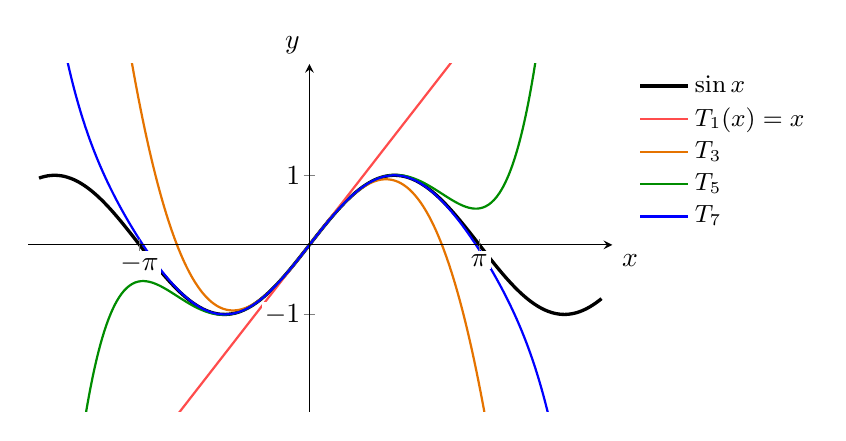
\begin{tikzpicture}
	\begin{axis}[
		axis lines=middle,
		xmin=-5.2, xmax=5.6,
		ymin=-2.4, ymax=2.6,
		xtick={-3.1416,3.1416}, xticklabels={$-\pi$,$\pi$}, ytick={-1,1}, tick label style={fill=white, inner sep=1pt}, axis on top,
		xlabel={$x$}, ylabel={$y$},
		xlabel style={below right}, ylabel style={above left},
		samples=200, smooth, clip=true,
		width=9cm, height=6cm,
		legend pos=outer north east, legend style={draw=none, fill=none, font=\small}, legend cell align=left
		]
		\addplot[very thick, black, domain=-5:5.4] {sin(deg(x))};
		\addlegendentry{$\sin x$}
		\addplot[thick, red!70, domain=-5:5.4] {x};
		\addlegendentry{$T_1(x)=x$}
		\addplot[thick, orange!90!black, domain=-5:5.4] {x-x^3/6};
		\addlegendentry{$T_3$}
		\addplot[thick, green!55!black, domain=-5:5.4] {x-x^3/6+x^5/120};
		\addlegendentry{$T_5$}
		\addplot[thick, blue, domain=-5:5.4] {x-x^3/6+x^5/120-x^7/5040};
		\addlegendentry{$T_7$}
	\end{axis}
\end{tikzpicture}
\end{document}
